%TODO mettere citazioni per Kim, Calandrino, Fedorova Chandra molka usando \cite
In most multicore platforms, different cores share onchip caches, usually is L2 or L3 cache. Recent research works show how an unfair cache sharing
among concurrent tasks and cache trashing degrades performance. Modern operating systems (OS), attempt to schedule threads in a
fair and low-overhead manner.
Most simply, they balance the load across processor by migrating task to keep the run queues approximately equal. An OS assumes that,
in a given timeslice, resource sharing uniformly impacts the rates of progress of all the co-scheduled threads.
Unfortunately this assumption is often unmet because a thread's ability to compete for cache space is determined by its temporal reuse behavior,
which is often very different compared to that of other threads which are co-scheduled with it.

An interesting work developed by S. Kim et al. shows the impact of an unfair cache sharing on performance and how this phenomena is dependent by
co-scheduled threads. In Figure \ref{fig:gzip_miss} is represented one of results provided by that work.

\begin{figure}[htbp]
\centering
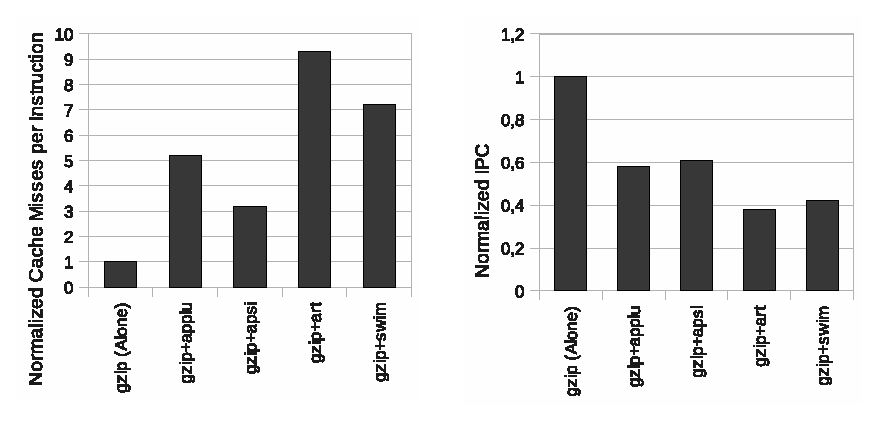
\includegraphics[width=\widefigure]{images/chandra_gzip}
\caption{\figurecaption{gzip miss rate}}
\label{fig:gzip_miss}
\end{figure}

The picture shows gzip's number of cache misses per instruction and instruction per cycle (IPC), when it runs alone compared to when it is
co-scheduled with different threads, such as applu, apsi, art, and swim. All the bars are normalized to the case where gzip is running alone.
It is interesting to note how gzip's number of cache misses per instruction increases significantly compared to when it runs alone. Infact, it increases 
by 3x when it runs with apsi and by 9.5x when it runs with art, 7.3x when it runs with swim.
Consequently, the IPC is affected differently. It is reduced by 35$\%$ when gzip runs with apsi, but reduced by 63$\%$ when gzip runs with art. 
Although not shown in the figure, art, apsi, applu, and swim's cache miss per instruction increases less than 15$\%$ when each of them runs with gzip. 

In terms of fairness, gzip's significant slow down can easily result in \textbf{priority inversion}. 
For example, if gzip has a higher priority than art, for gzip to achieve a higher progress rate, it has to be assigned more than three times the 
number of time slices compared to that assigned to art. Otherwise, to the end users, gzip may appear to be starved. In terms of throughput,
gzip's significant slow down reduces the overall throughput because the utilization of the processor where gzip runs on is also significantly reduced. 
Furthermore, it is possible that the co-scheduled threads's working sets severely overflow the cache and create a \textit{trashing} condition.

In briefly, there are at least three problems that may happen and render the OS schedule ineffective.
The first problem is \textit{thread starvation}, which happens when one thread fails in competing for sufficient cache space necessary to make 
satisfactory forward progress. The second problem is \textit{priority inversion}, where a higher priority thread achieves a slower forward
progress than a lower priority thread, despite the attempt by the OS to provide more timeslices to the higher priority thread.
This happens when the higher priority thread loses to the lower priority thread (or other threads) in competing for cache space. 
To make things worse, the operating system is not aware of this problem, and hence cannot correct this situation (by assigning more timeslices to the 
higher priority thread). The third problem is that the forward progress rate of a thread is \textit{highly dependent} on the thread mix in a co-schedule. 
This makes the forward progress rate difficult to characterize or predict, making the system behavior unpredictable. Unfortunately, despite these problems, 
cache implementations today are thread-blind, producing unfair cache sharing in many cases.

As I said in the first chapter, in theese years were developed some ideas about how to make a scheduler cache-aware.
This chapter aims to show the general structure and strategies used to model cache behaviour followed by theese algortihms, that are the most interesting 
part of theese type of heuristics.

%%%%%%%%%%%%%%%%%%%%%%%%%%%%%%%%%%%%%%%%%%%%%%%%%%%%%%%%%%%%%%%%%%%%%%%%%%%%%
\section{Structure of Cache aware Scheduling}

Before to explain how theese algortihms work, it is necessary to pay attention to which are assumptions made by theese heuristics about type of application 
and platform considered.

Assume a multicore platform consisting of $M$ cores that sharing an on-chip Last Level cache divided in $A$ partitions, and a task set $\tau$,
in which each task $T$ releases a job $J_i$ every period $p(T)$, and every released job is characterized by a worst-case execution time (WCET) denoted
by $e(T)$. This means that each job released by task $T$ has a maximum duration of $e(T)$. For each job is defined the number $A(J_k)$ that represents 
number of cache partitions, and then the total cache space size, used by it. For simiplicity we assume that each job generated by a task $T$ use the same
number of partition, therefore it is possbile to express $A(J_k)$ as $A(T)$.
The quantity $e(T)/p(T)$ is called the utilization of $T$, denoted $u(T)$. The deadline $d(J_k)$ of a job $J_k$ coincides with the release time of job 
$J_{k+1}$. If job $J_k$ completes its execution after time $d(J_k)$, then it is tardy. For some scheduling algorithms, tardiness may be bounded by some 
amount $B$, meaning that any job $J_k$ will complete execution no later than time $d(J_k)+B$. 

In this model we don't take care about core-local cache (usually L1) or other shared resources like interconnects are not modelled.
We assume the existence of a cache partitioning mechanism, allowing to divide the cache space into non-overlapping partitions. 
In this way, we know how many partitions, and then how many space, a task requires to execute its work. The model is very adapt to represent Real Time tasks.

\newpage

%-----------------------------------------------------------------------------
\subsection{The policy of the scheduler}

This kind of algorithms are a variant of classic scheduling algorithms, beacause they mantain the same characteristics, such as priority inheritance etc.,
and in addition they take care about which is memory region used by scheduled tasks. All heuristics analyzed follow theese rules: a job $J_k$ is 
scheduled for execution if:

\begin{enumerate}
	\item $J_k$ is the job of highest priority among all waiting jobs,
	\item There is at least one core idle
	\item There are enough cache partitions, i.e. at least $A(J_k)$ , are available.
\end{enumerate}

\begin{table}[htbp]
\begin{center}
\begin{tabular}{l|c|c|c}
	\hline
	& $p(T)$ & $C(T)$ & $A(T)$ \\ \hline
	$T_1$ & 3 & 2 & 1 \\ \hline
	$T_2$ & 4 & 3 & 2 \\ \hline
	$T_3$ & 5 & 3 & 2 \\ \hline
	$T_4$ & 8 & 3 & 1 \\ 
	\hline
\end{tabular}
\caption{An example task set}
\label{tab:cache_task_set}
\end{center}
\end{table}

\begin{figure}[htbp]
\centering
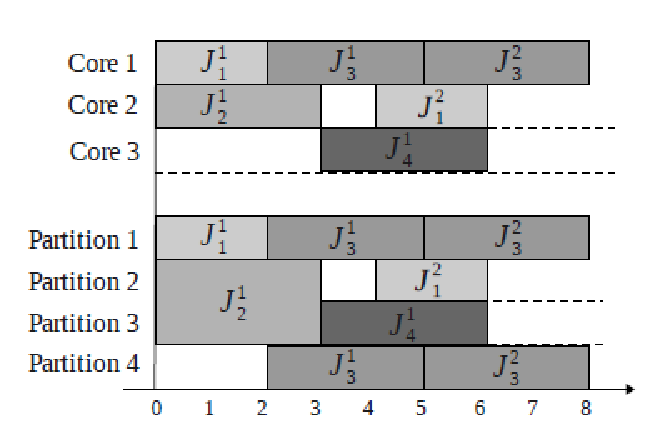
\includegraphics[width=\widefigure]{images/schedule.eps}
\caption{\figurecaption{Example of scheduling performed by cache aware policy}}
\label{fig:sched_example}
\end{figure}


Figure \ref{fig:sched_example} shows how the task set in Table \ref{tab:cache_task_set} is scheduled by our cache aware policy. The index of each task 
indentify the task and indicate the priority of the latter. Higher priority is 1 and lower priority is 4. In the picture jobs are represented in this way: 
$J_{\alpha}^\beta$, where $\alpha$ represents which task has released the job, and then also its priority, and $\beta$ is an index that identify the job.
At time 0 all jobs are released. At this time, the job $J_{4}^1$ can not be executed because it has lower priority than $J_{3}^1$ and the latter can not be
scheduled since there is not enough idle cache partitions available.

Analyzed algorithms implement this policy using different data structures and different strategies such as job promoting, variable time-slice etc., but 
the real differences between analyzed heuristics, are metrics and methods used to estimate which are the cache partitions requested by each task or
thread to schedule.

%-----------------------------------------------------------------------------
\section{Methods to infer cache space used}

As seen in the previous section, an hypotesis made in our application model is to have a mechanism, that we will call co-scheduler, that computes how many 
space each task requires. According to defined policy, the scheduler use theese informations and schedule tasks in order to avoid cache trashing.
In the development of this kind of scheduler, the real challange is to build an efficient co-scheduler that, at runtime, provides necessary informations.
In theese years, a lot of model to study cache behaviour in multicore systems were developed. In the majority, they are used as a profiling tool for
applications and not to implement cache aware scheduling heuristics %TODO ref al dynamic cache partition.
But some interesting works developed by Calandrino and Fedorova show how it is possible to build empirical and effective cache behaviour model
according to "low-cost" information suitable to implement a co-schedule systems. This works can be applied for both Real-time and general-purpose systems.

%-----------------------------------------------------------------------------
\subsection{Methods applied for Real-time systems}

Works developed by Calandrino et al. is focused on multimedia soft real-time application. In this work, tasks are multithreaded tasks applications (MTTs),
this hypotesis don't damage generality of the application model presented in the previous section.
Co-scheduler proposed is a profiler that provides a per-job working set sizes (WSS) estimate for each MTT. The per-job WSS of an MTT indicates the amount 
of memory referenced by all tasks of that MTT while executing one "job" of the MTT, where the ith job of an MTT consists of the ith jobs of all tasks 
in the MTT. It profiles MTTs rather than tasks since MTTs share a common working set. 
The profiling occurs during job execution, eliminating the need for and offline profiling tool. WSS may be seen as an oversimplification of 
cache behavior; but it to work well for small intervals (e.g., the execution time of a job). Further, it is usually the easiest metric to 
approximate efficiently given current hardware.

The profiler as stated requires some additional assumptions:

\begin{enumerate}
\item Each job of the same task is assumed to perform roughly the same operations on different (but similarly-sized) sets of data.
      This has two implications: (a) the ith job of task T and the j th job of task U , where T and U belong to the same MTT, do not share
      significant data unless i = j (even if T = U ); and (b) the per-job WSS of an MTT remains approximately the same over all jobs.

\item Profiled jobs are not preempted and do not cause shared cache thrashing.

\end{enumerate}

The first assumption is natural for certain types of (multimedia) applications. To ensure latter assumption, it is necessary discard measurements obtained
for jobs that are preempted, or for which cache thrashing occurred at some time during their execution. 
Thrashing is assumed to have occurred if for some quantum in which a job is scheduled, the sum of the WSSs of all MTTs with jobs scheduled in that quantum 
exceeds the shared cache size. For MTTs, measurements for the ith job of all thread in the MTT must be discarded if the $ith$ job of any thread in the 
MTT was preempted or caused thrashing.
Furthermore, the second assumption also implies that it is not interesting to profile MTTs with per-job WSSs greater than the size of the
shared cache, which would thrash the shared cache even if scheduled in isolation.

The above assumptions allow us to compute over all (non-discarded) jobs an average per-job MTT WSS, which it can be used as per-job WSS estimate for
an MTT. This can be computed by dividing the total shared cache misses observed over all profiled jobs by the total number of profiled jobs for an MTT, 
and multiplying the result by the cache line size.

But, how can it is possible to measure shared cache misses? Thanks to performance counters.
A performance counter for each core is programmed to track lower-level shared cache. Since jobs execute sequentially, it is possible to measure the number
of cache misses incurred for a job by resetting the counter to zero at the start of execution, and recording the total misses observed by the counter
upon completion. The observed misses can then be used to calculate a per-job WSS estimate. Since accessing program counters and recording data
are low-overhead operations, and computed WSS estimates are cached to minimize computation, the overhead of the profiler is relatively low.
It is clear that at the begin of a MTT, there isn't any measure about its miss rate. For this reason, profiler need of a initial tuning phase, in which an 
estimate of all MTT's WSS is done. This phase converge pretty fast to a reasonable result. For details see %TODO Calandrino 

%-----------------------------------------------------------------------------
\subsection{Methods applied for general purpose systems}

Co-scheduler developed by Fedorova et al. consider generic multithreaded tasks that can be preempted or not, it is not focused on soft Real-time 
applications. 

Their approach is based on an empirically observation that if the co-runners have similar cache miss rates they share the cache
roughly equally. So if co-runners A and B experience similar miss rates, they share the cache equally and they each experience their
\textbf{fair miss rate}. In this case, A and B are cache-friendly co-runners.

The fair miss rate is the number of misses per cycle (MPC) that would be generated by a thread if the cache were shared equally. This is metric used
to determine the best grouping between task.

Procedure to estimate the fair cache miss rate for each thread is very simple.
For each thread to profile, call it Thread A, execute it with several different co-runners and derive the relationship between its miss rate and 
miss rate of its corunner. This relationship is used to estimate the miss rate that Thread A would experience with a "hypothetical" 
cache-friendly co-runner; this miss rate is Thread A's fair miss rate. 

\newpage

\begin{figure}[htbp]
\centering
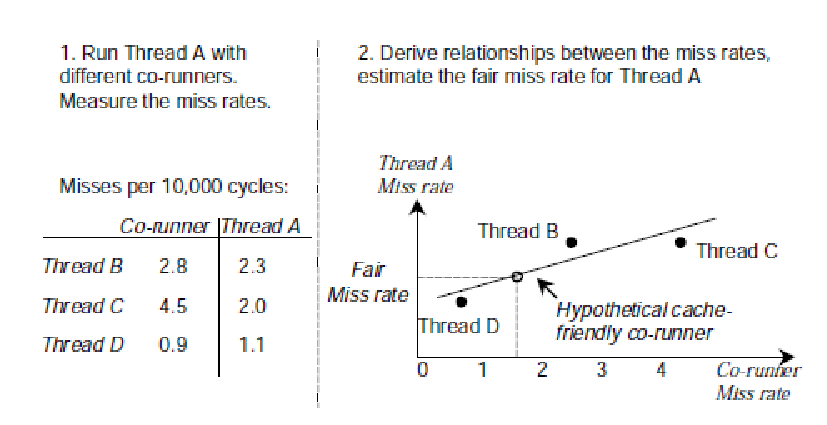
\includegraphics[width=\widefigure]{images/fedorova.eps}
\caption{\figurecaption{fedorova temp}}
\label{fig:fed}
\end{figure}

Figure \ref{fig:fed} illustrates this idea. Step 1 shows the miss rates measured as Thread A
runs with different co-runners. Step 2 shows that exists a linear relationship between the miss rate of Thread A and its co-runners.
We use the corresponding linear equation to compute Thread A's miss rate when running with a hypothetical cache-friendly co-runner - its fair miss 
rate.

This strategy is based on two important assumptions 
\begin {enumerate}
	\item Cache-friendly co-runners have similar cache miss rates.
	\item The relationship between co-runners' miss rates is linear.
\end{enumerate}

The former is true, because if each thread's shared cache accesses are uniformly distributed in the cache, it is possible to model cache 
replacement as a simple case of the balls in bins problem, that is: assume two co-runners, whose cache requests correspond to black and white balls 
respectively. We toss black and white balls into a bin. Each time a ball enters the bin, a ball is evicted from the bin. 
If we throw the black and white balls at the same rate, then the number of black balls in the bin after many tosses will form a
multinomial distribution centered around one-half. This result generalizes to any number of different colored balls being tossed at
the same rate. Thus, two threads with the same shared cache miss rate (balls being tossed at the same rate) will share the cache equally.
It is important to remark that this assumption is true only if cache request are uniformly distributed. Fedorova et al. have measured cache requested
made by SPEC2000 benchmarks, and they have found that for most benchmarks, the distribution was close to uniform, so it is correct using the balls in bins
problem to represent cache replacement

The latter assumption is demonstrated by this experiment.
They chose nine benchmarks from the SPEC CPU2000 suite with different cache access patterns and ran them in pairs on their simulated dual-core processor.
They ran each benchmark in several pairs. They analyzed the relationship between the miss rate of each benchmark and the miss rates of its co-runners and 
found that a linear equation approximated these relationships better than other simple functions.

The expression for the relationship between the co-runners' miss rates for a processor with $n+1$ cores is:
\begin{equation}
	MissRate(T) = a*\sum_{i=1} MissRate(C_{i}) + b
\label{eq:miss_rate}
\end{equation}

where,
\begin{enumerate}
	\item $T$ is a thread for which they compute the fair miss rate
	\item $C_i$ is the $i-th$ co-runner
	\item $n$ is the number of corunners
	\item $a$ and $b$ are the linear equation coefficients
\end{enumerate}

Thread $T$ experiences its fair cache miss rate $FairMissRate(T)$ when all concurrent threads experience the same miss rate, therefore:

\begin{equation}
	FairMissRate(T) = MissRate(T) = MissRate(C_i)
\end{equation}

for all $i$. Equation \ref{eq:miss_rate} can be expressed as:

\begin{equation}
	FairMissRate(T ) = a*n*FairMissRate(T) + b 
\end{equation}

where the expression for $FairMissRate(T)$ is:

\begin{equation}
	FairMissRate(T) = \frac {b}{1-a*n}
\end{equation}

The co-scheduler implemented dynamically derives coefficients for Equation 1 for each cache-fair thread at runtime and then estimates its fair cache 
miss rate. Also in this case, cache misses are retrived using performance counters, expressly programmed. Further, also this method requires a periodical 
tuning phase used to account thread's cache access pattern.

Showed approches are similar, but present some differences.
First of all, they are focused on two different type of tasks: first approach considers Real-Time tasks, the latter considers fair tasks.
Test environments are different. Calandrino et al work is Linux based, they used LITMUS benchmarks suite and they tested their work on Intel i7.
Fedorova et al. work is Solaris based, they used SPEC2000 benchmarks and they tested on a simulator of UltraSPARC T1
Both strategies try to understand how scheduled thread use shared cache, but they do this job in different way: the first method is focused only
to prevent cache trashing, the latter is more complex: it tries to prevent cache trashing too, furthermore it tries to understand how two co-scheduled
threads use shared cache.

Calandrino and Fedorova show in their papers how their works reduce shared cache miss and how this fact improve execution time (and predictability)
of benchmarks tested.

\section{Survey on cache architecture}
\label{sec:s1}

Over the years, cache architectures have always played an important role in system performance. Hundreds of research papers show how performance
can be improved using multi-level caches on a single-processor machine. Multicore systems introduce new challanges for cache designer, because cache memory 
is a shared resource, therefore issues related to how a core access to cached data and how the coherence regarding the access from different processors 
to the same cached data is guaranted are unavoidable. Furthermore, caches play an important role in managment of comunication betwen different core.
This section aims to show which are most important factors introduced in cache architecture to take in consideration during the development of cache aware
alogrithms from scratch. Theese cache characteristics are common in both general purpose and embedded systems.

%-----------------------------------------------------------------------------
\subsection{Cache coherent protocols}

Usually in multicore architecture, there is a private L1 cache for each core, and there is a L2 or L3 cache shared among all cores (SMP), or among cores 
that belong to the same node (NUMA). Shared cache is one of the most critical resources in multicores.

\begin{figure}[htbp]
\centering
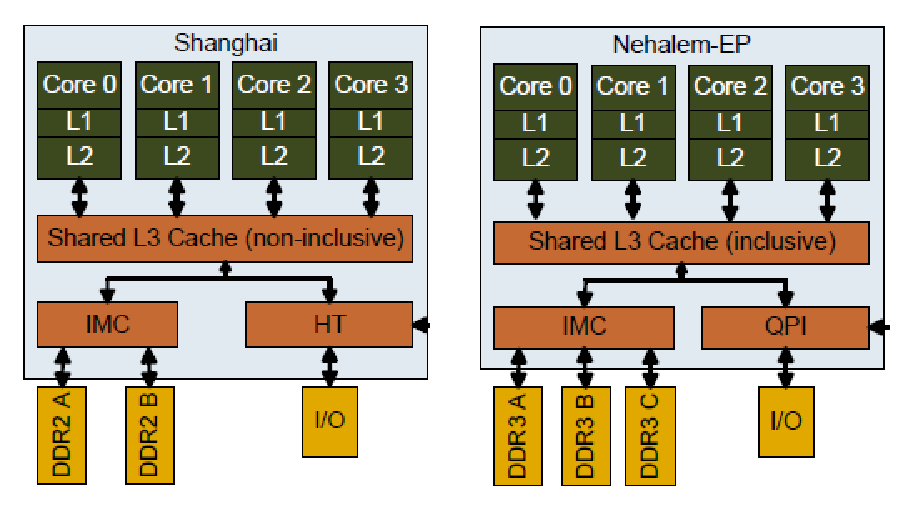
\includegraphics[width=\widefigure]{images/neh_amd.eps}
\caption{\figurecaption{Intel nehalem and AMD Shanghai}}
\label{fig:neh_amd}
\end{figure}

As for all types of shared resources, also for shared cache it's necessary to ensure integrity of the shared data.
Before to analyze mechanisms used to ensure data integrity, it is necessary pay attention to the difference between two terms: consistence and coherence.
When two or more CPUs operate on a shared variable and one of these CPUs modify the variable, it is necessary that the information regarding
this change of value be communicated to the other CPUs. Consistence refers to 'when' this change in memory data is available to other CPU cores.
Coherence refers to 'how' the change is communicated between the processors. Therefore, to ensure correctness of cache operations, it is necessary define
when a modified value must be made visible to another processor's read instruction, this is the consistency model, and define the rules used to comunicate 
memory update between different cores, this is coherence protocol. In briefly a cache coherence protocol is the mean used to maintains consistency between
all the cache in the system.
Existing coherence protocols are classified based on the mechanism by which they ensure cache coherence: 

\begin{itemize}

\item Snooping based protocols: Each cache monitors address lines of shared bus for every memory transaction made by remote processors. Appropriate action
is undertaken when data locally cached is modified by this transaction, for example: a write by a remote processor into a data address locally cached 
results in an invalidation of the local cache copy .

\item Snarfing based protocols: A cache controller watches both address and data in an attempt to update its own copy of a memory location when a second 
master modifies a location in main memory. When a write operation is observed to a location that a cache has a copy of, the cache controller updates its 
own copy of the snarfed memory location with the new data.

\item Directory-based protocols: Shared data are placed in a common directory that maintains the coherence between caches processor caches. 
This directory acts as a look-up table for every processor to verify coherence and consistency of data that is currently being read or updated.

\end{itemize}


The first two mechanisms are typical of the SMP architecture, while the last is used in large point-to-point inter-processor communication network 
architectures. Snooping protocols became popular and widely accepted with multiprocessors systems since it required minimal change to the pre-existing 
physical shared bus interface to the memory. The inherent broadcasting property of the snoop protocols makes it simple to implement but places an upper 
limit on scalability.
Over the years, several snooping based cache coherence protocols were developed. The most common is MESI protocol.
With this protocol, every cache line is marked with one of the following states:

\begin{itemize}

\item Modified
The cache line is present only in one of the local caches, and it has been modified from the value in main memory. Write on a modified cache line are 
allowed, reads are a bit complicated. The local cache that owns a modified cache line must intercept (snoop) all attempted reads (from all of the other 
caches in the system) at main memory location that correspond to modified cache line, forcing them to back off, then writing data to main memory and change
state of cache line to shared state.
 
\item Exclusive
The cache line is present only in the current cache, and it matches main memory. It is possible read/write lines in this state. A cache that own
line in exclusive state must snoop all read transaction from all other cache and if it intercepts some read that regard owned cache line, it changes
state of that line from exclusive to shared.

\item Shared
Indicates that this cache line may be stored in other caches and it matches the main memory. It is possible read cache line in this state. Writes to a shared
cache line are allowed but before to perform the operation, it is necessary invalidate all other copies in other caches.
A cache that holds a line in the Shared state must listen for invalidation from other caches, and discard the line (by moving it into Invalid state) on a 
match.

\item Invalid
Indicates that this cache line is invalid, read/write operation on invalid cache line are denied

\end{itemize}

Cache coherence protocols play an important role to improve efficiency of the read/write in cache. There are a lot of variant of MESI protocol, the most 
recent variants are MESIF and MOESI.

The former protocol adds Forward state. It is only relevant for the L3 cache. This state indicates that only one cache should act as a designated responder 
for any requests for the given line. With the standard MESI protocol, a request for cache line will receive a response from each cache that contains that 
line in the shared state. Instead, with MESIF protocol a request will be responded to only by the cache holding the line in the Forward state.
A cache line shared among multiple processors will be in forward state in only one L3 cache. This protocol is used in new Intel microarchitecture Nehalem 
and it is designed for ccNUMA. The aim of this new state is to reduce communications between cache.

The latter protocol add Owned state. A cache line in this state holds the most recent, correct copy of the data. Only one processor can hold the data 
in the Owned state, all other processors that contains a copy of that data must hold the them in the shared state. A copy of data in main memory can be 
incorrect. A cache line in owned state may be changed to the Modified state after invalidating all shared copies, or changed to the Shared state by 
writing the modifications back to main memory, furthermore cache lines must respond to a snoop request with data. 
It is clear that the aim of this protocol is to avoid the need to write a dirty cache line back to main memory when another processor tries to read it. 
With the Owned state, processor can supply the modified data directly to the other processor. This is beneficial when the communication latency and 
bandwidth between two CPUs is significantly better than to main memory. An example of MOESI implementation is present in AMD Shanghai microprocessor.

%-----------------------------------------------------------------------------
\subsection{Inclusive and exclusive cache}

Another important architecture detail that affect performance is if a cache is inclusive or exclusive.
An inclusive cache means that all data available in higher level cache are contained also in the last level cache, namely in shared cache.
An exclusive cache means that data is present only in one cache.

It is clear that theese two architectural policy are focused on two different aspects. The first policy greatly reduces snoop traffic because if a core 
doesn't find requested data in any of its cache level, it knows the data it is also not present in any other core's cache. The second policy, instead, 
allows to store more data than an inclusice cache, because for each data only one copy is stored.

An example of inclusive L3 shared cache is implemented in Intel Nehalem microarchitecture. In this implementation to insure coherency across 
all caches, the L3 cache line has additional flags that keep track of which core the data came from and a core valid bit that indicate that cache line 
is present in some core's cache. If the data is modified in L3 cache, then the L3 cache "knows" if the data came from a different core than last time 
and that the data in the first core needs its L1/L2 values updated with the new data. This greatly reduces the amount of traditional "snooping"
coherency traffic between cores. Moreover the core valid bit doesn't ensure that a L3 cache line is placed also in an higher level cache, because unmodified
cache lines may be evicted from a core's cache without notification of the L3 cache.

An implementation of exclusive cache can be found in AMD's Shanghai processors. Theese cpus present an interesting implementation of this type of cache
architecture, because L1 and L2 are exclusive cache, but last level shared cache (L3) is a not-inclusive cache.
Not-inclusive architecture is a variant of exclusive architecture, becasue if a cache line is transferred from the L3 cache into the L1 of any core, the 
line can be removed from the L3. According to AMD this happens if it is "likely" that the line is only used by one core, otherwise a copy can be kept in 
the L3.
About how the cpu can "understand" if a line will be used only by one core, AMD has not revealed details.
Nowadays, an inclusive cache is preferred over an exclusive cache, because it simplifies the problem of cache coherence. 

%-----------------------------------------------------------------------------
\subsection{Cache Hardware prefetcher}

It is necessary to spend a few words about prefetching. Prefetcher is an hardware component that tries to predict which memory addresses are
going to be used by the program, in order to load needed data in cache memory just in time.
Typical technical workloads often access memory in regular and sequential patterns, therefore, with a smart prediction mechanism, a prefetcher can select 
and load right data and, in this way, reduce memory latency. The key point to build a good prefetcher is to design prediction mechanism.
In literature there are many ideas to solve this problem. An example of concrete solution is the Intel Smart Memory access. This system was introduced
with Intel Core microarchitecture. In this system there are two prefetchers to the Level 1 data cache and the traditional prefetcher to the Level 1 
instruction cache. In addition there are two prefetchers associated with the Level 2 cache and shared between the cores. In total, there are eight
prefetchers per dual-core processor. 
In order to improve the accuracy of the prediction, the prefetcher system tags the history of each load using the Instruction Pointer (IP) of the load. 
For each load, the prefetcher builds a history and keeps it in a suitable history array. Based on load history, the prefetcher tries to predict the 
address of next load accordingly to a constant stride calculation (a fixed distance or "stride" between subsequent accesses to the same memory area). 
At this point, the prefetcher generates a prefetch request with the predicted address and brings the resulting data to the Level 1 data cache.
In literature, this kind of prefetchers are called \textit{strided} prefetcher.
Other architectures, such as Power ISA\_2.06, that use a strided prefetcher, introduces cache instructions to hint prefetch system for data prefetching.
With this instructions an application can specify direction, depth, no of units and so on. In this way, the programmer has a low level control on 
data prefetched.

Another category of prefetcher are \textit{non-strided} data prefetcher. They are very useful for accessing complex and irregular data structures as 
linked list, B-Trees etc. There are different techniques to implement theese prefetcher, one of theese is "pattern history based prefetcher". 
In this approach, the prefetcher tracks the addresses of misses and tries to identify specific patterns of misses that occur together (temporally). 
Once a pattern of misses has been detected, the prefetcher will find the first miss in the pattern. When this first miss occurs again, the prefetcher 
will immediately prefetch the rest of the pattern. For traversing a complex data structure like a linked list, this would be a fairly effective approach.
Recently AMD has announced that it will employs a non-strided prefetcher in its brand new Bulldozer microarchitecture, but it has not revealed details on 
implementations.

